\documentclass[journal]{IEEEtran}

% ---------------------------------------------------------------------------
% Preamble
%
% Built from scratch for this skeleton -- no prior main.tex existed anywhere
% on this machine or in this repository's history (confirmed via a full-disk
% search before writing this file), so there was nothing to "repair" in the
% literal sense. The brief's preamble-repair instructions (dedupe graphicx/
% booktabs/tabularx, drop subfigure/subcaption in favor of subfig alone,
% replace the IEEEtran \markboth demo placeholder, drop a non-functional
% \date) describe defects common to IEEEtran starter templates; this preamble
% is written to avoid all of them from the outset rather than to fix an
% existing file. See GPU_FREE_REPORT_2.md for this finding.
% ---------------------------------------------------------------------------

\usepackage{graphicx}
\usepackage{booktabs}
\usepackage{tabularx}
\usepackage{subfig}          % NOT subfigure or subcaption -- pick one, this is it
\usepackage{amsmath}
\usepackage{amssymb}
\usepackage{url}
\usepackage{xcolor}

\graphicspath{{../results/figures/}}

\begin{document}

\title{SpecAsync-UVM: Speculative Asynchronous Prefetch Infrastructure for the\\
NVIDIA Unified Virtual Memory Driver}

% TODO: draft -- author block. Names/affiliations/emails intentionally left
% as a placeholder; this is a structural skeleton only.
\author{%
  Author~Name,~\IEEEmembership{Member,~IEEE},
  Second~Author%
  \thanks{TODO: draft -- affiliation and contact footnote.}%
}

% No \date{} -- IEEEtran journal class does not use one; omitted rather than
% left as a stale non-functional placeholder.

\markboth{IEEE Transactions on XXXXXXXXXXXXXXXXXXXX,~Vol.~XX, No.~X, Month~2026}%
{Author \MakeLowercase{\textit{et al.}}: SpecAsync-UVM}

\maketitle

\begin{abstract}
% TODO: draft. See paper/abstract_v2.md for the current revised-abstract
% draft; the Gate 3 / Phase C conclusions (Path B closed, see
% results/phaseB2/GATE3_report.md and results/phaseC/PHASEC_REPORT.md) are
% not yet folded into that draft and must be before this abstract is
% finalized.
\end{abstract}

\begin{IEEEkeywords}
% TODO: draft -- keyword list.
\end{IEEEkeywords}

% =============================================================================
\section{Introduction}
\label{sec:introduction}
% TODO: draft. See paper/intro_revisions.md for drop-in replacement
% paragraphs (contribution list, motivation/hypothesis) already prepared
% against the Phase 1 results; these need revision against the Phase 2 /
% Gate 3 "Path B closed" finding before use here, per Task G's completeness
% ledger.

% =============================================================================
\section{Related Work}
\label{sec:related-work}
% TODO: draft. Citation audit and replacement BibTeX in
% results/analysis/BIB_AUDIT.md; do not cite anonymous2022learningoversub,
% jain2019crac, or bastemTilesTR under their current (miscited) metadata --
% use the corrected entries from that audit.

% =============================================================================
\section{Background: UVM Replayable Fault Handling}
\label{sec:background}
% TODO: draft. Source-level grounding for this section is in
% results/analysis/D5_CHARACTERIZATION.md (D1-D6 sub-phase definitions, call
% tree, and the file:line citations against the 595.71.05 tree).

% =============================================================================
\section{Design: SpecAsync Infrastructure}
\label{sec:design}
% TODO: draft. Producer-consumer ring, policy dispatch layer (adjacent-page,
% stride, Markov, oracle), debugfs telemetry interface. See
% paper/intro_revisions.md Replacement 1 for a drafted contribution
% description covering this section's content.

% =============================================================================
\section{Implementation}
\label{sec:implementation}
% TODO: draft. Module/patch structure: driver/patches/, driver/src/. Safety
% invariants preserved (see driver/PORTING_NOTES_595.md for v580->v595
% porting notes and API verification).

% =============================================================================
\section{Evaluation}
\label{sec:evaluation}

\subsection{Experimental Setup}
\label{sec:eval-setup}
% TODO: draft. Two platforms used across this project's phases: RTX 5070 Ti
% (Phase 1 / Gate 3, v595.71.05, Linux 6.14) and Tesla T4 / g4dn.xlarge
% (Phase C decomposition). See results/analysis/CLAIM_SCOPE.md for which
% claims are tied to which platform.

\subsection{Policy Sweep and the Decisive C0--C3 Comparison}
\label{sec:eval-policy-sweep}
% TODO: draft. Figure~\ref{fig:policy-matrix} (corrected Phase B policy
% sweep, pre-Gate-B.1-fix rows excluded per the exclusion manifest) and
% Figure~\ref{fig:decisive-c0c3} (Gate 3 C0-C3 distributions) are the primary
% evidence for this subsection. Statistical validation of the headline claim
% -- including where it does NOT hold and does not survive multiple-
% comparison correction -- is in results/analysis/STATISTICS.md,
% results/analysis/OUTLIER_FORENSICS.md, and
% results/analysis/MULTIPLE_COMPARISONS.md. Do not state the
% "statistically indistinguishable" claim as a blanket claim; it must be
% qualified per benchmark (see those files).

\begin{figure*}[t]
  \centering
  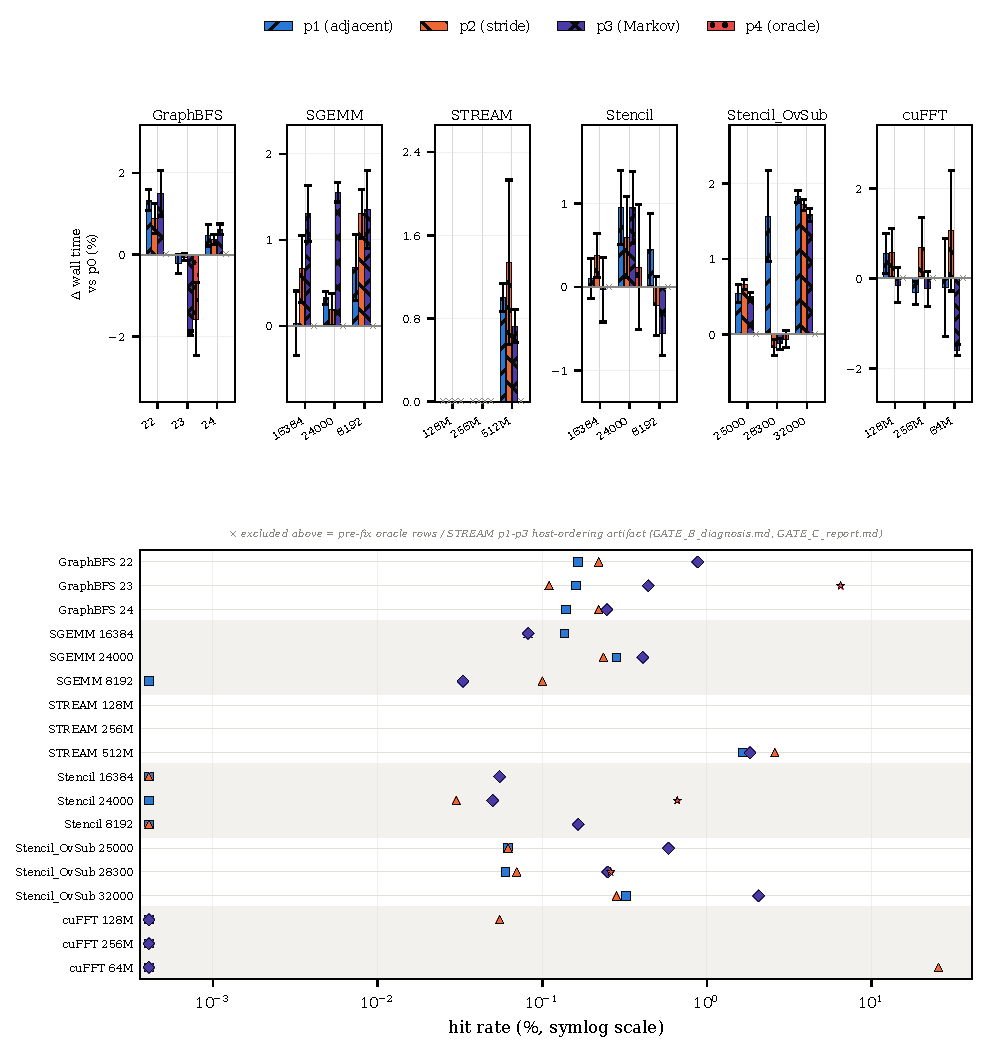
\includegraphics[width=\textwidth]{policy_matrix}
  \caption{\emph{TODO: draft caption.} Corrected Phase B policy sweep (p0-p4),
    excluding pre-Gate-B.1-fix oracle rows per
    results/figures/exclusion\_manifest.csv.}
  \label{fig:policy-matrix}
\end{figure*}

\begin{figure}[t]
  \centering
  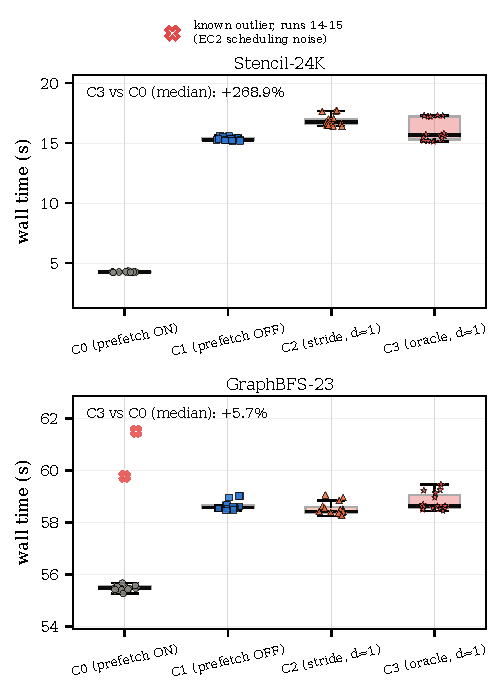
\includegraphics[width=\columnwidth]{decisive_c0c3}
  \caption{\emph{TODO: draft caption.} Gate 3 C0-C3 wall-time distributions,
    Stencil-24K and GraphBFS-23 (results/phaseB2/gate3/gate3\_times.csv).}
  \label{fig:decisive-c0c3}
\end{figure}

\subsection{Prefetch Opportunity vs.\ Cost}
\label{sec:eval-squeeze}
% TODO: draft. Figure~\ref{fig:the-squeeze} -- note that no prefetch-OFF
% real-benchmark hit-rate data exists anywhere on disk (documented, not
% estimated, in tools/figures/make_fig_the_squeeze.py's stdout output).

\begin{figure}[t]
  \centering
  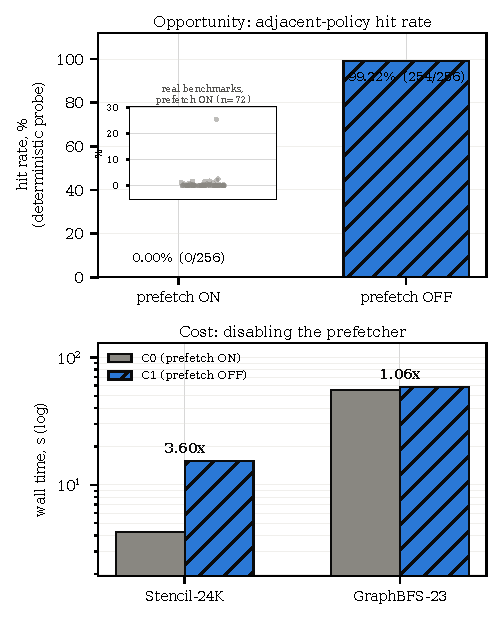
\includegraphics[width=\columnwidth]{the_squeeze}
  \caption{\emph{TODO: draft caption.} Panel A: synthetic probe hit rate
    (ON/OFF) vs.\ real-benchmark hit rates. Panel B: C0-vs-C1 wall-time
    ratio (results/phaseB2/gate3/gate3\_times.csv).}
  \label{fig:the-squeeze}
\end{figure}

\subsection{Oversubscription}
\label{sec:eval-oversub}
% TODO: draft. Figure~\ref{fig:oversub-collapse} -- oracle hit-rate collapse
% under 1.6x oversubscription (results/phaseB1/gate\_d/).

\begin{figure}[t]
  \centering
  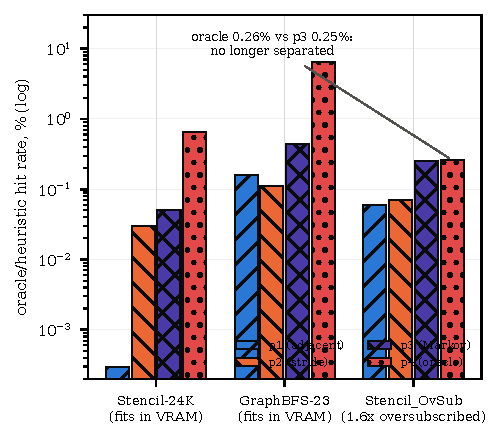
\includegraphics[width=\columnwidth]{oversub_collapse}
  \caption{\emph{TODO: draft caption.} Oracle/heuristic hit rate by regime and
    policy; oracle-vs-p3 separation collapses under oversubscription.}
  \label{fig:oversub-collapse}
\end{figure}

\subsection{Fault-Dispatch-Window Decomposition}
\label{sec:eval-decomposition}
% TODO: draft. Figure~\ref{fig:fault-density-sweep} -- absolute per-batch
% cost decomposition across the fault-density sweep
% (results/phaseC/PHASEC\_REPORT.md). D4/D5 dominance and its async-submit
% (not synchronous-wait) mechanism are established at the source level in
% results/analysis/D5_CHARACTERIZATION.md. The end-to-end wall-clock
% pipelining ceiling -- as opposed to the dispatch-window share reported
% here -- is NOT reliably computable for 6 of 7 workloads; see
% results/analysis/PIPELINING_CEILING.md before stating any single
% end-to-end percentage in this subsection.

\begin{figure}[t]
  \centering
  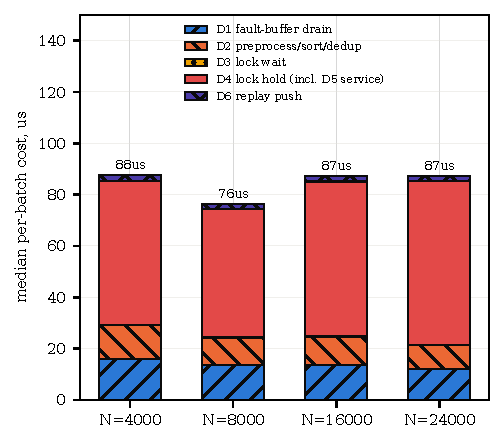
\includegraphics[width=\columnwidth]{fault_density_sweep}
  \caption{\emph{TODO: draft caption.} Median per-batch D1-D6 decomposition
    (absolute \textmu s) across the Phase C fault-density sweep
    (N=4000/8000/16000/24000).}
  \label{fig:fault-density-sweep}
\end{figure}

\begin{table}[t]
  \centering
  \caption{\emph{TODO: draft caption.} Gate 3 decisive comparison, n=15/cell
    (results/phaseB2/gate3/gate3\_times.csv; see
    results/analysis/STATISTIC\_OF\_RECORD.md for the median-as-statistic-
    of-record declaration these numbers should use).}
  \label{tab:gate3-summary}
  \begin{tabularx}{\columnwidth}{l l X X X}
    \toprule
    Config & Benchmark & Median (s) & vs.\ C0 & vs.\ C1 \\
    \midrule
    % TODO: draft -- populate from results/phaseB2/gate3/gate3_times.csv
    % via results/analysis/STATISTIC_OF_RECORD.md's verified deltas.
    \multicolumn{5}{c}{\itshape (table body not yet populated)} \\
    \bottomrule
  \end{tabularx}
\end{table}

\subsection{Cross-Platform Confirmation (RTX 5070 Ti vs.\ Tesla T4)}
\label{sec:eval-cross-platform}
% TODO: draft narrative prose. Data table populated below from
% results/analysis/GATE_B5_5070TI_REPLICATION.md (Task B, Part 3 work
% block) -- T1's exact pre-registered interleaved protocol
% (results/analysis/PREREGISTRATION.md), rerun unmodified on a second,
% architecturally-different GPU (RTX 5070 Ti, Blackwell, driver 595.84)
% against a freshly-collected oracle trace (not T4's). Two results
% reproduce (Path-B-closed magnitude order, Stencil-24K C3-vs-C1
% significance); two do NOT reproduce (GraphBFS-23's C3-vs-C1 null,
% Stencil-24K's C3 bimodal pattern) -- see the source report for exact
% numbers and the honest treatment of both divergences. Do not draft this
% subsection's prose from a stale/partial reading of the table alone;
% integrate the source report's per-comparison detail.

\begin{table}[t]
  \centering
  \caption{\emph{TODO: draft caption.} T1's interleaved C0--C3 protocol
    (n=20/cell, kept phase), Tesla T4 vs.\ RTX 5070 Ti. Absolute medians are
    not cross-platform-comparable (see
    results/analysis/GATE\_B5\_5070TI\_REPLICATION.md); the delta\% and
    Holm-significance columns are the comparable quantities.}
  \label{tab:cross-platform-t1}
  \begin{tabularx}{\columnwidth}{l l X X X X}
    \toprule
    Comparison & Bench & T4 $\Delta\%$ & T4 Holm & 5070Ti $\Delta\%$ & 5070Ti Holm \\
    \midrule
    C3 vs C0 & Stencil-24K & +278.5\% & Yes & +302.3\% & Yes \\
    C3 vs C0 & GraphBFS-23 & +7.34\% & Yes & +4.83\% & Yes \\
    C3 vs C1 (primary) & Stencil-24K & +6.67\% & Yes & +3.60\% & Yes \\
    C3 vs C1 (primary) & GraphBFS-23 & +0.02\% & \textbf{No} & $-$0.39\% & \textbf{Yes} \\
    C2 vs C1 & Stencil-24K & +8.22\% & Yes & +3.71\% & Yes \\
    C2 vs C1 & GraphBFS-23 & $-$0.24\% & Yes & $-$0.47\% & Yes \\
    \bottomrule
  \end{tabularx}
\end{table}

% =============================================================================
\section{Discussion}
\label{sec:discussion}
% TODO: draft. Draft sentences for methodology-level nuances (median-of-
% ratios vs.\ ratio-of-medians, the D3 "no lock pressure" caveat, the
% GraphBFS C2-vs-C1 anomaly) are pre-drafted in
% results/analysis/STATISTIC_OF_RECORD.md and
% results/analysis/GRAPHBFS_C2_ANOMALY.md respectively -- integrate rather
% than redraft.

% =============================================================================
\section{Limitations and Threats to Validity}
\label{sec:limitations}
% TODO: draft. Candidate content: the five measurement artifacts catalogued
% in results/analysis/ARTIFACT_CATALOG.md (and how each was caught); the
% claim-scope split (driver-architectural vs.\ platform-specific-cost-ratio)
% in results/analysis/CLAIM_SCOPE.md; the Gate-3 run-ordering limitation
% (only C2-vs-C1 has drift control between its two arms) from
% results/analysis/OUTLIER_FORENSICS.md \S{}1; the cuFFT single-platform
% hedge from results/figures/CUFFT_PROVENANCE.md.

% =============================================================================
\section{Conclusion}
\label{sec:conclusion}
% TODO: draft.

% =============================================================================
% \nocite{*} forces every ref.bib entry to appear in the bibliography even
% though no section body cites anything yet (this is a prose-free skeleton).
% This exists ONLY to exercise the bibtex/IEEEtran.bst toolchain end-to-end
% for the build-verification step -- remove it once real \cite{} calls exist
% in the drafted section bodies.
\nocite{*}
\bibliographystyle{IEEEtran}
\bibliography{ref}

\end{document}
